% Prof. Dr. Ausberto S. Castro Vera
% UENF - CCT - LCMAT - Curso de Ci\^{e}ncia da Computa\c{c}\~{a}o
% Campos, RJ,  2022
% Disciplina: An\'{a}lise e Projeto de Sistemas
% Aluno: Luiz Miguel Guedes Gomes

\chapterimage{analise.png} % Table of contents heading image
\chapter{Etapa de An\'{a}lise}

Neste cap\'{\i}tulo descrevemos...

\textbf{Hardware}
\begin{itemize}[label={}]
	\item \textbf{1. Computadores em todas as unidades}
		\subitem 1.1. Em cada unidade deverá haver pelo menos um computador no caixa
	\item \textbf{2. Tablets em todas as unidades}
		\subitem 2.1. Em cada unidade deverá haver pelo menos um tablet por setor frequentado pelos clientes
	\item \textbf{3. Equipamento de comunicação entre funcionários}
		\subitem 3.1. A comunicação à distância entre os funcionários poderá ser feita por alto falantes ou dispositivos móveis.
	\item \textbf{4. Monitores para os computadores}
		\subitem 4.1 Em cada unidade deverá existir pelo menos um monitor para cada computador
	\item \textbf{5. Boa visibilidade do televisor central da unidade}
		\subitem 5.1. O televisor central deverá ser uma Smart TV de 40 polegadas ou maior*
	\item \textbf{6. Segurança de linha}
		\subitem 6.1. Em cada unidade deverão ser utilizados filtros de linhas, nobreaks e estabilizadores em conjunto para evitar a influência de oscilações no fornecimento de energia, a qual podem prejudicar a funcionalidade e longevidade do sistema
	\item \textbf{7. Disponibilidade de internet}
		\subitem 7.1. Em cada unidade deverá existir pelo menos um roteador de rede wireless por setor e/ou alance máximo do sinal de outro roteador
		\subitem 7.2. Todos os computadores devem possuir placas de rede wireless embutido
	\item \textbf{8. Servidores dedicados}
		\subitem 8.1. Em pelo menos uma unidade deverá existir pelo menos um servidor para hospedagem do site do sistema
		\subitem 8.2. Em pelo menos uma unidade deverá existir pelo menos um servidor para hospedagem do banco de dados do sistema
	\item \textbf{9. Refrigeração da sala de servidores}
		\subitem 9.1 A sala dos servidores deverá se manter sempre refrigerada por meio de ar-condicionados
	\item \textbf{10. Impressão de relatórios e documentos fiscais}
		\subitem 10.1 O sistema deverá contar com impressoras para imprimir documentos e relatórios importantes para a organização institucional
	\item \textbf{11. Mobílias ergonômicas}
		\subitem 11.1 O sistema deverá contar com mobílias ergonômicas que possibilitem o bem estar de seus usuários
	\item \textbf{12. Sistemas de segurança}
		\subitem 12.1. O sistema deverá contar com pelo menos uma câmera por setor, de forma que cubra os principais pontos do ambiente e seus principais equipamentos
		\subitem 12.2. O sistema também deverá contar com um sistema de armazenamento das gravações das câmera, sendo este feito fisicamente e/ou na nuvem 
		\subitem 12.3. Os produtos deverão ser equipados com sensores antifurto simples e a prova d'água que possam ser removidos e recolocados em outros produtos
		\subitem 12.4. As salas principais de equipamento e a sala dos servidores deverá contar com controle de acesso por meio de leitores de digital ou de íris e portas automatizadas
		\subitem 12.5. Toda câmera e equipamento fora da sala principal deverá ser protegido por grade caso esteja sujeito a furto e julgado desprotegido 
	\item \textbf{13. Recursos de acessibilidade}
		\subitem 13.1. Os tablets distribuídos pela unidade devem contar com displays que possibilitem a boa leitura e compreensão das informações
		\subitem 13.2. Os tablets da unidade também deverão ser distribuídos em locais de fácil acesso a todas as pessoas, principalmente às que possuem dificuldade de locomoção e visão. 
		\subitem 13.3. Controle de itinerário dos funcionários 
\end{itemize}
\textbf{Software}
\begin{itemize}[label={}]
	\item \textbf{1. Acesso ao sistema}
		\subitem 1.1 O acesso ao sistema pelos usuários deverá ser feito por meio de nome do usuário ou e-mail e senha, biometria ou 	      
leitor de íris
			\subsubitem 1.1.1 Abir interface inicial de acesso em uma janela do aplicativo, programa ou website
			\subsubitem 1.1.2 Inserir informações de acesso (nome do usuário ou e-mail, senha, biometria ou leitura de íris) 
			\subsubitem 1.1.3 Caso tenha sido usada a biometria ou leitura de íris deverão ser puladas as próximas duas etapas
			\subsubitem 1.1.4 Verificar usuário cadastrado 
			\subsubitem 1.1.5 Verificar senha cadastrada
			\subsubitem 1.1.6 Liberar área e ferramentas de trabalho
			\subsubitem 1.1.7 Permitir acesso à internet
			\subsubitem 1.1.8 Fazer controle hierárquico de acesso do usuário ao sistema
			\subsubitem 1.1.9 Finalizar processo
	\item \textbf{3. Cadastro de produto}
		\subitem 3.1 Todos os novos produtos adquiridos deverão ser cadastrado no banco de dados do sistema
	\item \textbf{4. Controle de usuários}
		\subitem 4.1 O sistema deverá contar com um sistema de hierarquia entre os usuários, onde clientes, funcionários, gerentes e fornecedores terão acesso a diferentes ferramentas e restrição de acesso a outros recursos pertencentes a usuários de maior grau administrativo.**
	\item \textbf{8. Controle de estoque}
		\subitem 8.1 A entrada e saída de mercadoria da unidade, seja por compra, ganho, venda ou descarte, deverá ser computados no banco de dados do sistema, afim de evitar imprecisões nos cálculos administrativos da empresa**
	\item \textbf{9. Interface amigável}
		\subitem 9.1 O sistema deverá contar com uma interface agradável aos usuários, buscando seguir padrões já conhecidos e usados pelos usuários como modelo
	\item \textbf{10. Recursos de acessibilidade}
	\begin{itemize}[label={}]
		\item 10.1 Os equipamentos que possuam display e que estejam em constante comunicação com os usuários, deverá contar com recursos no software que possibilitem a acessibilidade de pessoas deficientes 
			\subitem 10.1.1 Se aproximar do equipamento
			\subitem 10.1.2 Caso necessário solicitar os seguintes recursos de acessibilidade por comando de voz, gestos ou touch:
				\subsubitem   10.1.2.1 Recurso de ampliação de imagem e textos
				\subsubitem   10.1.2.2 Recurso de audiodescrição
				\subsubitem   10.1.2.3 Recurso de descrição por libras
			\subitem 10.1.3 Caso as necessidades estejam satisfeitas pular a próxima etapa
			\subitem 10.1.4 Caso haja algum problema, chamar algum outro funcionário por meio do próprio equipamento ou outra forma adequada
			\subitem 10.1.5 Finalizar processo
	\end{itemize}
	\item \textbf{11. Backup diário}
		\subitem 11.1 O sistema deverá contar com backups diários, quer sejam armazenados na nuvem, quer sejam armazenados de forma local, de forma a evitar perdas importantes nos dados e alterações relevantes no sistema
	\item \textbf{12. Versionamento do website}
		\subitem 12.1 O sistema deverá contar com um organizado sistema de versionamento do website, a fim de auxiliar o processo de desenvolvimento do mesmo, a constante adaptação e evolução, assim como garantir backup de versões e recursos antigos
		\subitem 12.2 Os desenvolvedores, arquitetos de software e analistas devem usar mesmo método de versionamento, tendo o mesmo programa instalado e utilizando a mesma plataforma de hospedagem de código-fonte e arquivos com controle de versão
			\subsubitem 12.2.1 Abrir arquivo alterado em seu programa de desenvolvimento de códigos-fonte ou arquivos
			\subsubitem 12.2.2 Verificar se está alterando a versão desejada
			\subsubitem 12.2.3 Abrir o console para digitar os comandos desejados
			\subsubitem 12.2.4 Utilizar a ramificação em que se deseja submeter alterações
			\subsubitem 12.2.5 Caso seja necessário, utilize comandos para alterar a ramificação atual para a desejada
			\subsubitem 12.2.6 Identificar a forma de submissão desejada
			\subsubitem 12.2.7 Digitar o comando de submissão
			\subsubitem 12.2.8 Escrever a mensagem de alteração de forma descritiva e de fácil compreensão
			\subsubitem 12.2.9 Submeter alterações
			\subsubitem 12.2.10 Finalizar o processo
	\item \textbf{13. Versionamento do aplicativo}
		\subitem 13.1 O sistema deverá contar com um organizado sistema de versionamento do aplicativo, a fim de auxiliar o processo de desenvolvimento do mesmo, a constante adaptação e evolução, assim como garantir backup de versões e recursos antigos
		\subitem 13.2 Os desenvolvedores, arquitetos de software e analistas devem usar mesmo método de versionamento, tendo o mesmo programa instalado e utilizando a mesma plataforma de hospedagem de código-fonte e arquivos com controle de versão
			\subsubitem 13.1.1 Abrir arquivo alterado em seu programa de desenvolvimento de códigos-fonte ou arquivos
			\subsubitem 13.1.2 Verificar se está alterando a versão desejada
			\subsubitem 13.1.3 Abrir o console para digitar os comandos desejados
			\subsubitem 13.1.4 Utilizar a ramificação em que se deseja submeter alterações
			\subsubitem 13.1.5 Caso seja necessário, utilize comandos para alterar a ramificação atual para a desejada
			\subsubitem 13.1.6 Identificar a forma de submissão desejada
			\subsubitem 13.1.7 Digitar o comando de submissão
			\subsubitem 13.1.8 Escrever a mensagem de alteração de forma descritiva e de fácil compreensão
			\subsubitem 13.1.9 Submeter alterações
			\subsubitem 13.1.10 Finalizar o processo
	\item \textbf{28. Informações privilegiadas à fornecedores}
		\subitem 28.1. O sistema poderá fornecer informações privilegiadas à fornecedores cadastrados de forma seletiva, como disponibilidade de produto no estoque, demanda por produto, orçamento para encomendas e valor estipulado para encomenda
			\subsubitem 28.1.1. Abir interface inicial de acesso em uma janela do aplicativo, programa ou website
			\subsubitem 28.1.2. Inserir informações de acesso (nome do usuário ou e-mail, senha, biometria ou leitura de íris)
			\subsubitem 28.1.3. Caso tenha sido usada a biometria ou leitura de íris deverão ser puladas as próximas duas etapas
			\subsubitem 28.1.4. Verificar usuário cadastrado 
			\subsubitem 28.1.5. Verificar senha cadastrada
			\subsubitem 28.1.6. Liberar área e ferramentas de trabalho
			\subsubitem 28.1.7. Permitir acesso à internet
			\subsubitem 28.1.8. Fazer controle hierárquico de acesso do usuário ao sistema
			\subsubitem 28.1.9. Fornecer informações selecionadas para aquele fornecedor
			\subsubitem 28.1.10. Disponibilizar meios de submeter propostas e orçamentos de produtos
			\subsubitem 28.1.11. Disponibilizar essa propostas caso sejam submetidas, para o setor financeiro, afim de analisá-las
			\subsubitem 28.1.12. Acompanhar andamento do processo
			\subsubitem 28.1.13. Caso seja validade a proposta, fornecer recursos para negociar e estabelecer data e hora de entrega
			\subsubitem 28.1.14. Finalizar processo
	\item \textbf{30. Manutenção de perfis nas redes sociais}
		\subitem 30.1. A rede de comércio deverá contar com perfis nas redes sociais que divulguem o nível de satisfação dos clientes com o sistema, dicas de uso do site e do aplicativo, divulgação de promoções exclusivas, entre outras publicações que visem melhorar a imagem pública e confiabilidade de antigos e novos clientes da marca 
	\item \textbf{32. Sistema avaliativo (serviços e produtos)}
		\subitem 32.1. O sistema deverá contar com um método avaliativo opcional aos usuários sobre qualidade de serviço e produtos, assim como grau de recomendação sobre determinada mercadoria
			\subsubitem 32.1.1. Abir interface inicial de acesso em uma janela do aplicativo, programa ou website
			\subsubitem 32.1.2. Inserir informações de acesso (nome do usuário ou e-mail, senha, biometria ou leitura de íris)
			\subsubitem 32.1.3. Caso tenha sido usada a biometria ou leitura de íris deverão ser puladas as próximas duas etapas
			\subsubitem 32.1.4. Verificar usuário cadastrado 
			\subsubitem 32.1.5. Verificar senha cadastrada
			\subsubitem 32.1.6. Liberar área e ferramentas de trabalho
			\subsubitem 32.1.7. Permitir acesso à internet
			\subsubitem 32.1.8. Fazer controle hierárquico de acesso do usuário ao sistema
			\subsubitem 32.1.9. Disponibilizar recursos avaliativos de produtos já adquiridos
			\subsubitem 32.1.10. Disponibilizar meios de submeter fotografias 
			\subsubitem 32.1.11. Enviar fotografias submetidas para avaliação automatizada e humana 
			\subsubitem 32.1.12. Caso seja validado a segurabilidade moral da fotografia e conformidade com o contexto, submeter para visibilidade pública no site e aplicativo
			\subsubitem 32.1.13. Finalizar processo
		\subitem 32.2. O sistema também poderá contar com um meio de submissão de fotografias de clientes dos produtos adquiridos que já estejam em suas residências, incentivando novas compras**
			\subsubitem 32.2.1. Abir interface inicial de acesso em uma janela do aplicativo, programa ou website
			\subsubitem 32.2.2. Inserir informações de acesso (nome do usuário ou e-mail, senha, biometria ou leitura de íris)
			\subsubitem 32.2.3. Caso tenha sido usada a biometria ou leitura de íris deverão ser puladas as próximas duas etapas
			\subsubitem 32.2.4. Verificar usuário cadastrado 
			\subsubitem 32.2.5. Verificar senha cadastrada
			\subsubitem 32.2.6. Liberar área e ferramentas de trabalho
			\subsubitem 32.2.7. Permitir acesso à internet
			\subsubitem 32.2.8. Fazer controle hierárquico de acesso do usuário ao sistema
			\subsubitem 32.2.9. Disponibilizar recursos avaliativos de produtos já adquiridos 
			\subsubitem 32.2.10. Analisar avaliações a fim de evitar comentários ofensivos
			\subsubitem 32.2.11. Caso seja validado a segurabilidade moral do comentário submeter para visibilidade pública no site e aplicativo
			\subsubitem 32.2.12. Finalizar processo
	\item \textbf{40. Banco de dados automatizado}
	\begin{itemize}[label={}]
		\item 40.1. O banco de dados deverá ser inter comunicativo com o gerenciador de saída e de entrada de mercadorias do estoque, assim como com o registro de entrada e saída de funcionários através do relógio de ponto e leitores de biometria ou íris 
			\subitem 40.1.1. Verificar comunicação com rede wireless dos sensores, leitores e do relógio de ponto
			\subitem 40.1.2. Inicializar programa de gerenciamento de banco de dados
			\subitem 40.1.3. Executar o script que deverá submeter os dados adquiridos de tais equipamentos para o banco de dados, sendo que este deverá: 
				\subsubitem 40.1.3.1. Receber as informações coletadas
				\subsubitem 40.1.3.2. Processá-las de forma a se moldarem no formato dos dados aceitos pelo banco de dados
				\subsubitem 40.1.3.3. Enviá-los para o programa gerenciador de banco de dados
			\subitem 40.1.4. O programa de gerenciamento de banco de dados deverá ser configurado para organizar as informações recebidas cada qual em sua determinada área, de forma organizada e correta
			\subitem 40.1.5. Finalizar processo
	\end{itemize}
\end{itemize}
\textbf{Pessoas}
\begin{itemize}[label={}]
	\item \textbf{9. Equipe de instalação/manutenção especializada}
		\subitem 9.1. A equipe de instalação/manutenção deverá cotar com profissionais nas área de eletroeletrônica, assim como na área de instalação e manutenção de hardware e software
	\item \textbf{11. Equipe treinada para operação do sistema} 
		\subitem 11.1. A equipe de antigos e novos funcionários deverá ser apta a operar pelo menos o básico do novo sistema contratado, a fim de aproveitar ao máximo os recursos disponibilizados para auxiliar os mesmos na sua rotina laboral
\end{itemize}
\textbf{Banco de dados}
\begin{itemize}[label={}]
	\item \textbf{1. Armazenamento de informações administrativas no banco de dados}
		\subitem 1.1. O banco de dados deverá registrar informações sobre: 
			\subsubitem 1.1.1. Funcionários
			\subsubitem 1.1.2. Estoque
			\subsubitem 1.1.3. Clientes
			\subsubitem 1.1.4. Compras e vendas
			\subsubitem 1.1.5. Encomendas
			\subsubitem 1.1.6. Entregas
			\subsubitem 1.1.7. Promoções
			\subsubitem 1.1.8. Produtos
			\subsubitem 1.1.9. Produtores
			\subsubitem 1.1.10. Fornecedores
			\subsubitem 1.1.11. Preços
			\subsubitem 1.1.12. Avaliações e comentários
	\item \textbf{2. Dados fiscais e financeiros}
		\subitem 2.1. O banco de dados deverá auxiliar na geração de documentos fiscais e elaboração de orçamentos 
	\item \textbf{4. Automação do banco de dados}
		\subitem 4.1. O banco de dados deverá se comunicar com o gerenciador de saída e de entrada de mercadorias do estoque, com o registro de entrada e saída de funcionários através do relógio de ponto, com o caixa, a fim de registrar todos os movimentos empresariais na rede, facilitando assim os processos administrativos e fiscais
\end{itemize}
\textbf{Mobilidade}
\begin{itemize}[label={}]
	\item 1. Disponibilidade 
		\subitem 1.1. O sistema deverá contar com disponibilidade em todos os principais dispositivos móveis, seja por meio do aplicativo ou pelo website 
\end{itemize}
\section{Requisitos do Sistema}
\textbf{Hardware}
\begin{enumerate}
	\item Computadores em todas as unidades
	\item Tablets em todas as unidades
	\item Equipamento de comunicação entre funcionários
	\item Monitores para os computadores
	\item Boa visibilidade do televisor central da unidade
	\item Segurança de linha
	\item Disponibilidade de internet
	\item Servidores dedicados
	\item Refrigeração da sala de servidores
	\item Impressão de relatórios e documentos fiscais
	\item Mobílias ergonômicas
	\item Sistemas de segurança
	\item Recursos de acessibilidade
\end{enumerate}
\textbf{Software}
\begin{enumerate}
	\item Acesso ao sistema
	\item Cadastro de clientes
	\item Cadastro de produto
	\item Controle de usuários
	\item Edição de documentos
	\item Salvar documentos
	\item Registro de vendas
	\item Controle de estoque
	\item Interface amigável 
	\item Recursos de acessibilidade
	\item Backup diário
	\item Versionamento do website
	\item Versionamento do aplicativo
	\item Tolerância a falhas
	\item Disponibilidade de produtos
	\item Segurança dos bancos de dados
	\item Segurança dos dados da empresa
	\item Proteção contra vírus 
	\item Compras online
	\item Encomendas online
	\item Informações sobre produtos
	\item Rastreio de entrega de produtos
	\item Sistema de gerenciamento de finanças
	\item Geração de relatórios automatizados
	\item Acesso ao pacote Office 
	\item Sistema operacional proprietário atualizado 
	\item Segurança no sistema de pagamento 
	\item Informações privilegiadas à fornecedores
	\item Divulgação nas redes sociais 
	\item Manutenção de perfis nas redes sociais
	\item Ambiente interativo entre clientes
	\item Sistema avaliativo (serviços e produtos)
	\item Divulgação de promoções 
	\item Acesso ao sistema facilitado por biometria
	\item Programa calculador de tendência de compra
	\item Programa gerador de orçamentos da empresa
	\item Calculador de desconto
	\item Comparador de preços 
	\item Atualização do banco de dados
	\item Banco de dados automatizado
	\item Intercomunicação de dados entre as unidades
	\item Contabilizar horas de trabalho de funcionários 
	\item Sistema inteligente de recompensas aos funcionários
	\item Programa auxiliar de declaração de imposto de renda
\end{enumerate}
\textbf{Pessoas}
\begin{enumerate}
	\item Gerente de projeto
	\item Gerente de segurança
	\item Analista de projeto
	\item Arquitetos de software
	\item Equipe de desenvolvedores devidamente instruídos
	\item Designers de website 
	\item Designers de aplicativo
	\item Operadores de banco de dados contextualizados
	\item Equipe de instalação/manutenção especializada
	\item Técnicos de rede 
	\item Equipe treinada para operação do sistema
\end{enumerate}
\textbf{Documentação}
\begin{enumerate}
	\item Manual do usuário
	\item Manual do sistema
	\item Catálogo digital dos produtos (disponíveis, já vendidos e encomendáveis)
	\item Emissão de nota fiscal 
	\item Disponibilidade de dados atualizados para declaração de imposto de renda**(funcionário, encomendas, saída, gastos, lucros,etc)
	\item Relatórios (automáticos e impressos)
	\item Guia básico de uso (para cada usuário)
\end{enumerate}
\textbf{Banco de dados}
\begin{enumerate}
	\item Armazenamento de informações administrativas no banco de dados
	\item Dados fiscais e financeiros
	\item Programa gerenciador de banco de dados
	\item Automação do banco de dados
\end{enumerate}
\textbf{Procedimentos e metodologia}
\begin{enumerate}
	\item Treinamentos
	\item Instalações
	\item Manutenção mensal
	\item Backups diários
	\item Cadastro de usuário
\end{enumerate}
\textbf{Mobilidade}
\begin{enumerate}
	\item Disponibilidade 
	\item Recursos auxiliares mobile aos funcionários
	\item Tablets pelo estabelecimento
	\item Aplicativo mobile
	\item Website 
\end{enumerate}
\textbf{Nuvem}
\begin{enumerate}
	\item Backup de dados
	\item Uso de computação de borda*
	\item Hospedagem auxiliar do sistema na nuvem
\end{enumerate}

\section{Stakeholders e Pontos de Vista}

Nesta seção serão apresentados os públicos alvo do sistema, os chamados stakeholders. Da mesma forma, também serão descritos os diferentes pontos de vista em relação ao sistema e os serviços que se relacionarão aos mesmos.

\subsection{Stakeholders}
\begin{itemize}
	\item Clientes 
	\item Funcionários
	\item Fornecedores
	\item Entregadores
	\item Produtores
	\item Gestores financeiros
	\item Gerentes de negócio das unidades
	\item Proprietário(s) da rede de comércio
	\item Acionistas
	\item Departamento de marketing
	\item Equipe de instalação/manutenção 
	\item Gerente de segurança
	\item Técnicos de rede
	\item Operador de banco de dados
	\item Técnicos em Eletroeletrônica
\end{itemize}

\subsection{Pontos de vista e serviços}
\textbf{Diretos:}
\begin{itemize}
	\item Clientes 
		\subitem-- Cadastro
		\subitem -- Compras online
		\subitem -- Pesquisa de produtos
		\subitem -- Verificação de promoções
		\subitem -- Histórico de compras
		\subitem -- Contas a pagar
		\subitem -- Métodos avaliativos de produtos e serviços
		\subitem -- Catálogo de produtos
		\subitem -- Notificações 
		\subitem -- Rastreio de entrega
		\subitem -- Acesso à internet
		\subitem -- Informações sobre os produtos
		\subitem -- Interface amigável e responsiva 
		\subitem -- Segurança de dados
		\subitem -- Confiabilidade nos serviços 
		\subitem -- Confiabilidade nos métodos de pagamento
		\subitem -- Acessibilidade ao sistema
		\subitem -- Encomendar
	\item Funcionários
		\subitem-- Cadastro
		\subitem -- Carga horária de trabalho cumprida e restante 
		\subitem -- Conquistas 
		\subitem -- Relatórios
		\subitem -- Interface amigável e responsiva 
		\subitem -- Histórico de vendas
		\subitem -- Tarefas
		\subitem -- E-mail
		\subitem -- Pesquisa de produtos
		\subitem -- Catálogo de produtos
		\subitem -- Notificações 
		\subitem -- Rastreio de entrega de vendas
		\subitem -- Rastreio de entrega de subsídio
		\subitem -- Informações sobre os produtos
		\subitem -- Segurança de dados
		\subitem -- Acesso à internet
		\subitem -- Confiabilidade na plataforma
		\subitem -- Verificação de promoções
		\subitem -- Histórico de preços
		\subitem -- Cadastrar clientes
		\subitem -- Acessibilidade ao sistema
		\subitem -- Maior nível de usuário
		\subitem -- Encomendar
		\subitem -- Gerenciar encomendas
	\item Equipe de instalação/manutenção 
		\subitem -- Cadastro
		\subitem -- Estado dos equipamentos
		\subitem -- Acesso remoto ao sistema
		\subitem -- Acesso à internet
		\subitem -- Avaliação sobre sistema e serviços
		\subitem -- Relatórios 
		\subitem -- Planta atualizada da unidade
		\subitem -- Versão dos softwares
		\subitem -- Versão dos hardwares
		\subitem -- Acesso físico ao sistema
	\item Técnicos de rede
		\subitem -- Cadastro
		\subitem -- Controle de PCs
		\subitem -- Controle de Tablets
		\subitem -- Controle de usuários
		\subitem -- Controle de servidores
		\subitem -- Acesso remoto ao sistema
		\subitem -- Acesso físico ao sistema
		\subitem -- Esquema de distribuição de rede na unidade
		\subitem -- Sub-redes
		\subitem -- Histórico de uso de rede
	\item Operador de banco de dados
		\subitem -- Cadastro
		\subitem -- Acesso ao sistema
		\subitem -- Acesso ao programa de gerenciamento de banco de dados
		\subitem -- Faturas
		\subitem -- Receitas
		\subitem -- Despesas
		\subitem -- Orçamentos
		\subitem -- Histórico de vendas
		\subitem -- Histórico de encomendas
		\subitem -- Carga horária cumprida por funcionários
		\subitem -- Itinerário do funcionário durante expediente 
		\subitem -- Acesso à internet
		\subitem -- E-mail
		\subitem -- Tarefas
		\subitem -- Taxa de venda de produtos
		\subitem -- Histórico de preços
		\subitem -- Contas a receber
		\subitem -- Contas a pagar
		\subitem -- Débitos a clientes
		\subitem -- Liquidação de contas
		\subitem -- Informações sobre estoque
		\subitem -- Controle de entrada e saída de mercadoria 
		\subitem -- Notas fiscais de vendas
		\subitem -- Segurança de dados
		\subitem -- Relatórios
		\subitem -- Confiabilidade na plataforma
		\subitem -- Maior nível de usuário
\end{itemize}
\textbf{Indiretos:}
\begin{itemize}
	\item Proprietário(s) da rede de comércio
		\subitem -- Cadastro
		\subitem -- Faturas
		\subitem -- Receitas
		\subitem -- Despesas
		\subitem -- Orçamentos
		\subitem -- Acesso à internet
		\subitem -- Taxa de venda de produtos
		\subitem -- Rendimento dos funcionários
		\subitem -- Relatórios
		\subitem -- Gerenciamento de reuniões
		\subitem -- Interface amigável e responsiva 
		\subitem -- Segurança de dados
		\subitem -- Confiabilidade na plataforma
	\item Acionistas
		\subitem -- Cadastro
		\subitem -- Receitas
		\subitem -- Despesas
		\subitem -- Orçamentos
		\subitem -- Acesso à internet
		\subitem -- Gerenciamento de reuniões
		\subitem -- Relatórios
		\subitem -- Taxa de venda de produtos
		\subitem -- Rendimento dos funcionários
		\subitem -- Interface amigável e responsiva 
		\subitem -- Segurança de dados
		\subitem -- Confiabilidade na plataforma
	\item Gerentes de negócio das unidades
		\subitem -- Faturas
		\subitem -- Receitas
		\subitem -- Despesas
		\subitem -- Orçamentos
		\subitem -- Histórico de vendas
		\subitem -- Histórico de encomendas
		\subitem -- Rendimento dos funcionários
		\subitem -- Carga horária cumprida por funcionários
		\subitem -- Acesso à internet
		\subitem -- Interface amigável e responsiva 
		\subitem -- E-mail
		\subitem -- Gerenciamento de reuniões
		\subitem -- Tarefas
		\subitem -- Taxa de venda de produtos
		\subitem -- Histórico de preços
		\subitem -- Itinerário do funcionário durante expediente 
		\subitem -- Avaliação dos produtos e serviços 
		\subitem -- Relatórios
		\subitem -- Informações sobre estoque
		\subitem -- Segurança de dados
		\subitem -- Confiabilidade na plataforma
		\subitem -- Maior nível de usuário
	\item Gestores financeiros
		\subitem -- Contas a receber
		\subitem -- Contas a pagar
		\subitem -- Débitos a clientes
		\subitem -- Liquidação de contas
		\subitem -- Boletos bancários
		\subitem -- E-mail
		\subitem -- Gerenciamento de reuniões
		\subitem -- Faturas
		\subitem -- Receitas
		\subitem -- Despesas
		\subitem -- Orçamentos
		\subitem -- Informações sobre estoque
		\subitem -- Acesso à internet
		\subitem -- Interface amigável e responsiva 
		\subitem -- Histórico de vendas
		\subitem -- Notas fiscais de vendas
		\subitem -- Segurança de dados
		\subitem -- Relatórios
		\subitem -- Confiabilidade na plataforma
		\subitem -- Histórico de preços
		\subitem -- Acessibilidade ao sistema
		\subitem -- Maior nível de usuário
	\item Departamento de marketing
		\subitem -- Acesso à internet
		\subitem -- Acesso às redes sociais
		\subitem -- Conquistas 
		\subitem -- Taxa de venda de produtos
		\subitem -- Interface amigável e responsiva 
		\subitem -- Histórico de vendas
		\subitem -- Informações sobre estoque
		\subitem -- Pesquisa de produtos
		\subitem -- Catálogo de produtos
		\subitem -- Informações sobre os produtos
		\subitem -- Verificação de promoções
		\subitem -- Histórico de preços
	\item Gerente de segurança
		\subitem -- Cadastro
		\subitem -- Estado dos equipamentos
		\subitem -- Acesso remoto ao sistema
		\subitem -- Acesso físico ao sistema
		\subitem -- Acesso à internet
		\subitem -- Planta atualizada da unidade
		\subitem -- Gerenciamento de reuniões
		\subitem -- Acesso às câmeras
		\subitem -- Armazenamento das câmeras
		\subitem -- Itinerário do funcionário durante expediente 
		\subitem -- Informações sobre estoque
		\subitem -- Controle de entrada e saida de mercadoria 
		\subitem -- Controle de entrada e saida de pessoas
		\subitem -- Controle de comunicação
		\subitem -- Controle de usuários
		\subitem -- Inventário
	\item Entregadores
		\subitem-- Cadastro
		\subitem -- Relatórios
		\subitem -- Visualizar encomendas
		\subitem -- Histórico de entregas
		\subitem -- Tarefas
		\subitem -- Pesquisa de produtos
		\subitem -- Catálogo de produtos
		\subitem -- Acesso à internet
		\subitem -- Notificações 
		\subitem -- Rastreio de entrega
		\subitem -- Informações sobre os produtos
		\subitem -- Segurança de dados
		\subitem -- Confiabilidade na plataforma
		\subitem -- Acessibilidade ao sistema
		\subitem -- Interface amigável e responsiva 
	\item Fornecedores
		\subitem -- Cadastro
		\subitem -- Orçamentos disponibilizados 
		\subitem -- Interface amigável e responsiva 
		\subitem -- Histórico de encomendas entregues
		\subitem -- Nível do estoque
		\subitem -- Pesquisa de produtos
		\subitem -- Catálogo de produtos
		\subitem -- Pedido de reuniões
		\subitem -- Notificações 
		\subitem -- Rastreio de entrega de encomendas
		\subitem -- Informações sobre os produtos
		\subitem -- Segurança de dados
		\subitem -- Avaliações sobre produto
		\subitem -- Confiabilidade na plataforma
		%\subitem -- Histórico de preços
		\subitem -- Acessibilidade ao sistema
	\item Produtores
		\subitem -- Cadastro
		\subitem -- Orçamentos disponibilizados 
		\subitem -- Interface amigável e responsiva 
		\subitem -- Histórico de venda de produtos
		\subitem -- Nível do estoque
		\subitem -- Pesquisa de produtos
		\subitem -- Catálogo de produtos
		\subitem -- Notificações 
		\subitem -- Pedido de reuniões
		\subitem -- Informações sobre os produtos
		\subitem -- Segurança de dados
		\subitem -- Avaliações sobre produto
		\subitem -- Taxa de venda do produto
		\subitem -- Confiabilidade na plataforma
		\subitem -- Acessibilidade ao sistema
\end{itemize}

\section{Entrevista}

A entrevista é uma técnica importante e a mais usada forma de coleta de requisitos para um sistema. Foram selecionadas 6 perguntas que serão realizadas, para o entendimento do sistema antigo e para possíveis melhorias para o novo sistema. A entrevista será feita com um funcionário no cargo de atendente do setor de atendimento. Foi escolhido o funcionário do setor de atendimento pelo fato de ser o setor que mais utiliza o sistema.

\begin{enumerate}
	\item \textbf{O que acha do sistema atual?}
		\subitem r: O sistema atual é muito lento e atrapalhado no atendimento, além de ser muito rudimentar, ou seja, não combina muito com a realidade em que vivemos, com tantas inovações tecnológicas. 
	\item \textbf{Qual a sua maior dificuldade com o atual sistema?}
		\subitem r: A nossa maior dificuldade são os horários de pico, onde muitos clientes fazem muitas perguntas ao mesmo tempo sobre as plantas e outras mercadorias e nós não conseguimos responder adequadamente.
	\item \textbf{Quais são melhorias que você gostaria de ver em relação ao atendimento?}
		\subitem r: Gostaria de ter uma forma de o cliente se atender sozinho, ver informações sobre o produto sem precisar do funcionário o tempo todo ao seu lado.
	\item \textbf{Quais são melhorias que você gostaria de ver em relação à segurança?}
		\subitem r: Gostaria de ter algo que impeça furtos quando estamos distraídos em outras tarefas, para poder nos concentrar no nosso atendimento e serviço, como alarmes, sensores, etc. 
	\item \textbf{Você utiliza todas as funções do sistema atual?}
		\subitem r: Tem coisas que eu faço do meu jeito, tem outras que só os técnicos conseguem fazer, o sistema é muito complicado e a gente foi pouco instruído a usá-lo.
	\item \textbf{O que você adicionaria no novo sistema?}
		\subitem r: Eu adicionaria um catalogo mais detalhado sobre os produtos, com disponibilidade, fotos e informações, pra facilitar o fornecimento de informações ao cliente e agilizar o atendimento.
\end{enumerate}

\section{ Casos de Uso}
Nesse capítulo serão apresentados os casos de uso do sistema, a fim de representar descritivamente e visualmente as interações realizadas pelos usuários com o sistema as respostas do mesmo.
\subsection{Diagramas de caso de uso}
\begin{table}[H]
	    \begin{center}
	    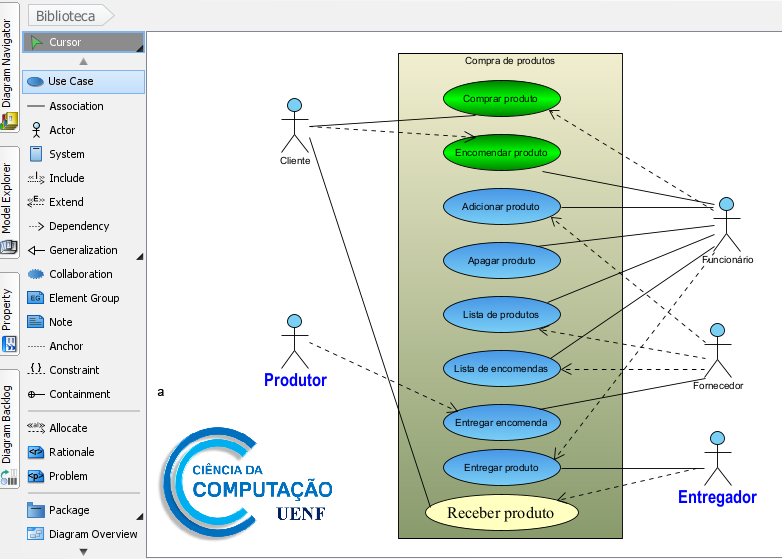
\includegraphics[width=14cm]{caso_de_uso.png}
	    \caption{Caso de uso mais recorrente} \label{tab:casoUso}
	    \end{center}
\end{table} 

\section{Modelagem do Sistema}
\subsection{Modelagem de Dados: Diagramas de fluxo de dados}
Na seção a seguir serão representadas graficamente as interações entre processos e bases de dados do sistema. 

	\subsubsection{3.5.1.1 Diagrama de contexto}
	 O diagrama a seguir tem por objetivo apresentar um panorama geral de todo sistema, assim como seus objetivos e funções gerais.
	 \begin{table}[H]
	 \begin{center}
	    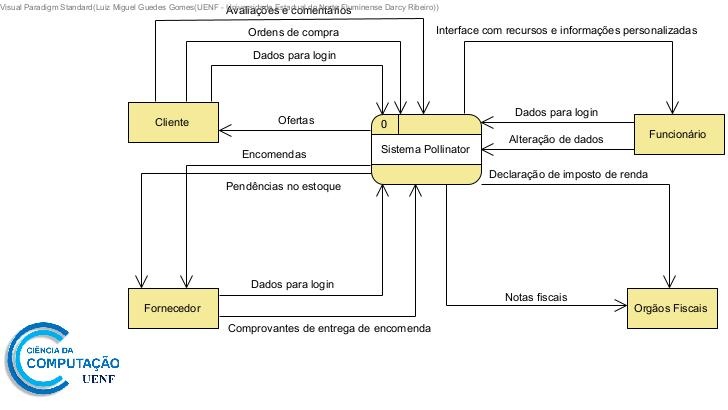
\includegraphics[width=14cm]{DFD1.jpg}
	    \caption{Diagrama de contexto} \label{tab:DFD1}
	 \end{center}
	 \end{table} 
	\subsubsection{3.5.1.2 Diagrama do sistema}
 Os diagramas a seguir tem por objetivo apresentar o sistema por completo, com todas as funções e subfunções, assim como os fluxos de dados que os compõem e todas as bases de dados envolvidas.
 	\begin{table}[H]
	 \begin{center}
	    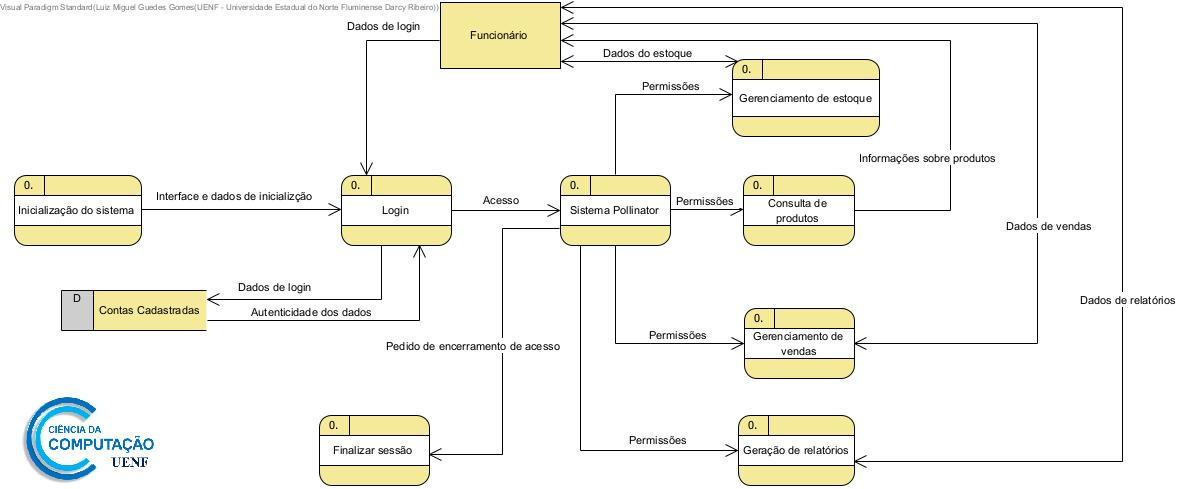
\includegraphics[width=14cm]{DFD2.jpg}
	    \caption{Diagrama do sistema: Login de funcionários ao sistema Pollinator } \label{tab:DFD2}
	 \end{center}
	 \end{table} 
	 
	 \begin{table}[H]
	 \begin{center}
	    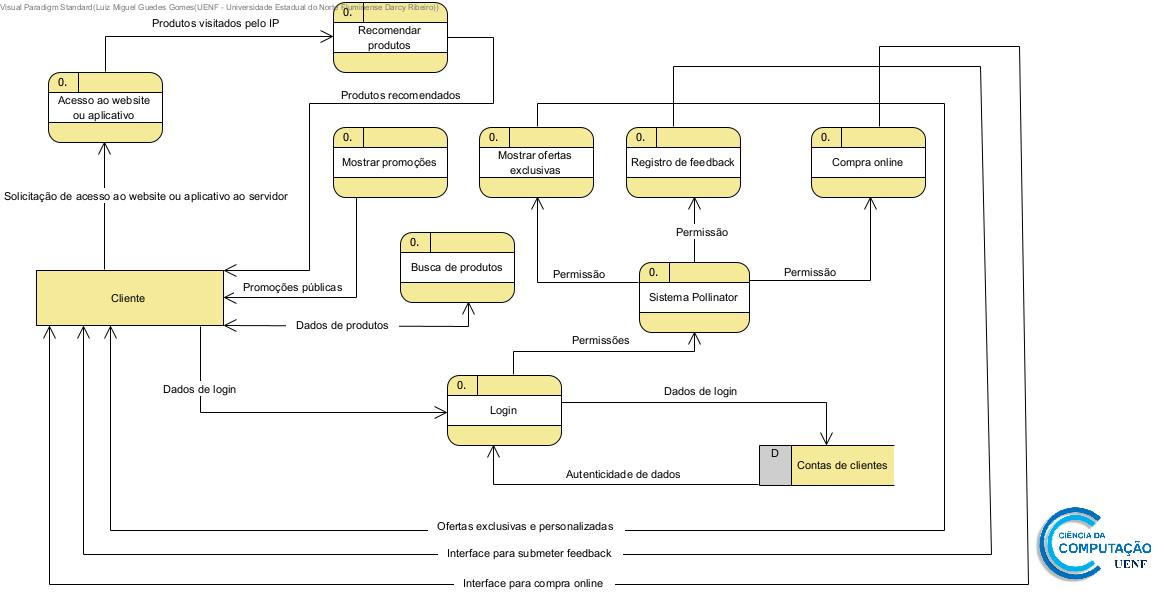
\includegraphics[width=14cm]{DFD3.jpg}
	    \caption{Diagrama do sistema: Login dos clientes ao sistema Pollinator } \label{tab:DFD3}
	 \end{center}
	 \end{table} 
	 
\subsection{Modelagem de Processos}
 	Os diagramas de processos apresentados nessa seção têm o intuito de fornecer uma
visão ampliada das funções de alguns recursos do sistema.

	\begin{table}[H]
	 \begin{center}
	    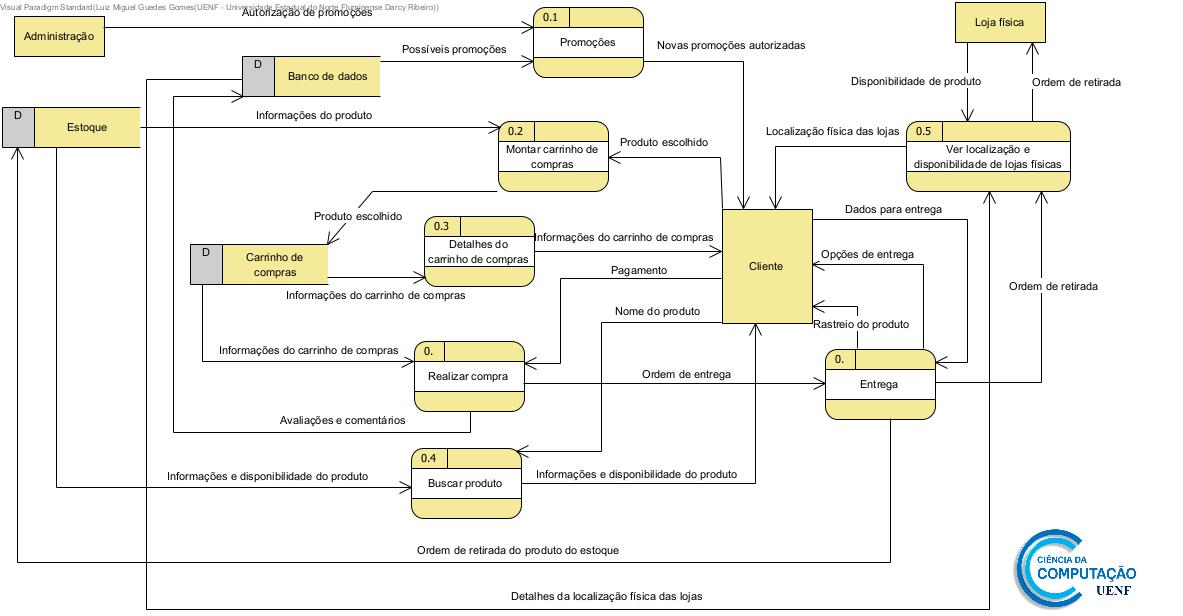
\includegraphics[width=14cm]{DFD4.jpg}
	    \caption{Diagramas de processos: Sistema de compra online e auto-atendimento} 
	 	\label{tab:DFD4}
	 \end{center}
	 \end{table} 
	 
	 \begin{table}[H]
	 \begin{center}
	    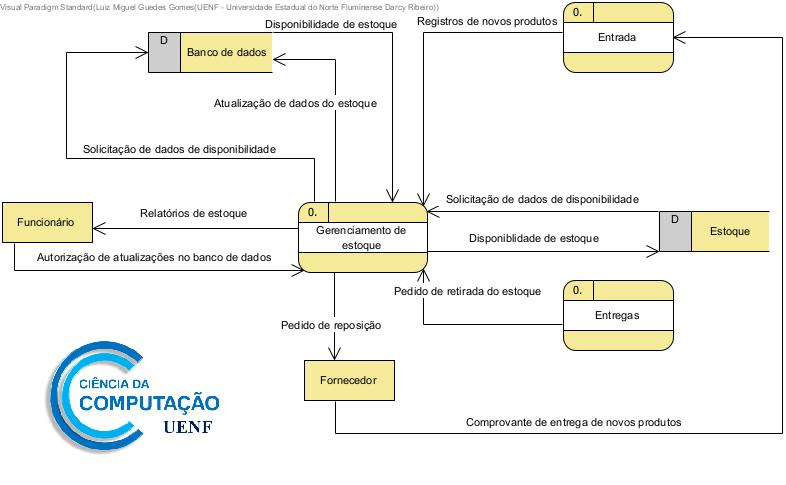
\includegraphics[width=14cm]{DFD5.jpg}
	    \caption{Diagramas de processos: Gerenciamento de estoque } 						\label{tab:DFD5}
	 \end{center}
	 \end{table} 
	 

\subsection{Modelagem de entidades e relacionamentos}
	Os diagramas a seguir ilustram o relacionamento entre as diferentes entidades que interagem direta ou indiretamente com o sistema. Os relacionamentos modelados são os entre os clientes, o sistema e os funcionários(3.7), entre o cliente e o sistema para compras online(3.8) e entre a administração, o sistema de acusação de possíveis promoções e a exibição dessas promoções aos clientes(3.9).
	\begin{table}[H]
	 \begin{center}
	    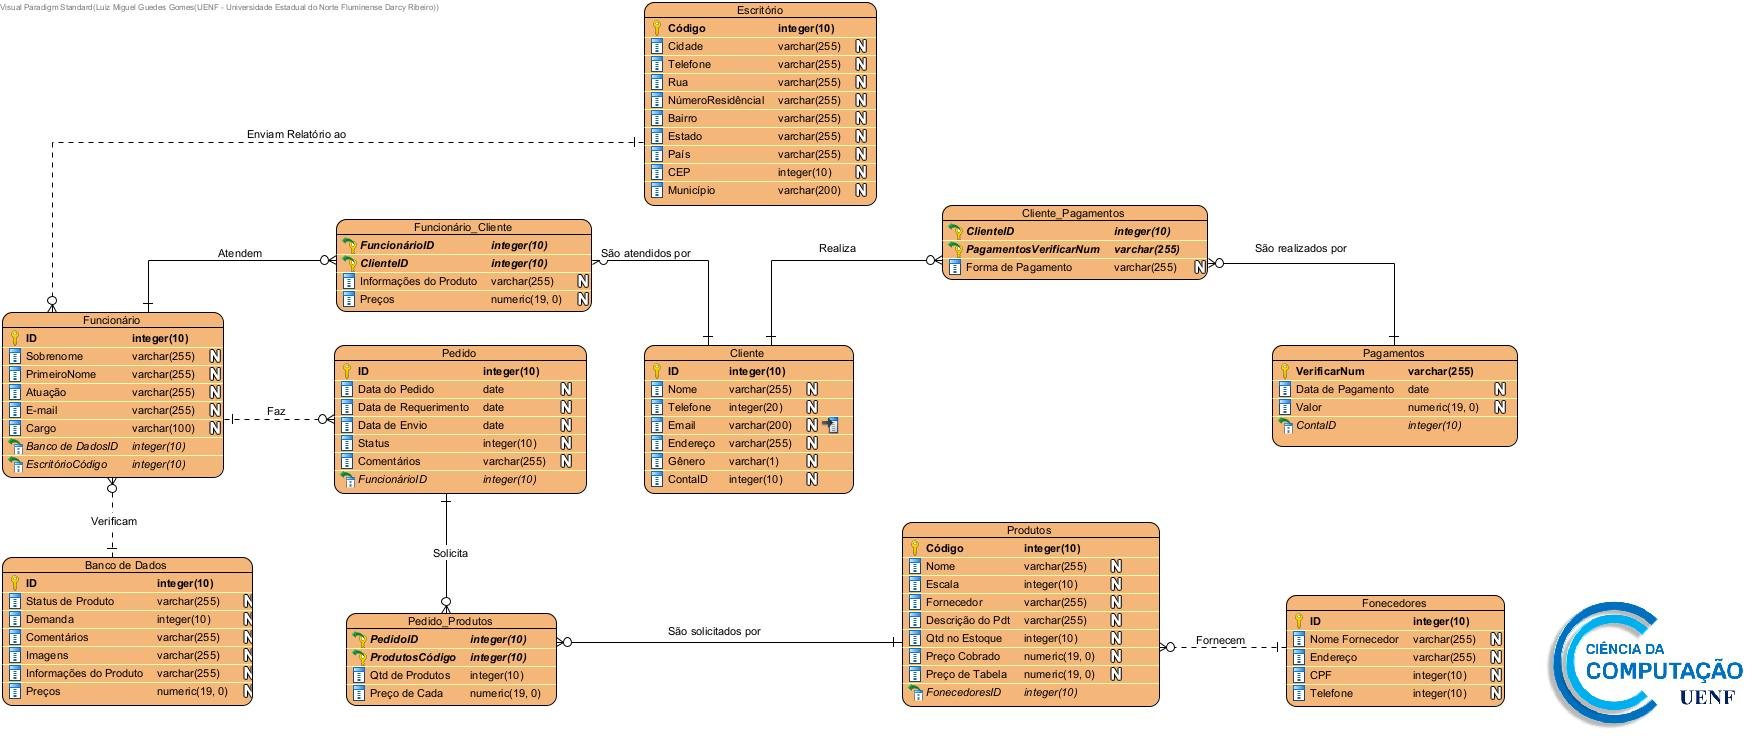
\includegraphics[width=14cm]{DFD6.jpg}
	    \caption{Diagrama de Relacionamento:Cliente-Sistema-Funcionário} 		
	    \label{tab:DFD6}
	 \end{center}
	 \end{table} 
	 
	 \begin{table}[H]
	 \begin{center}
	    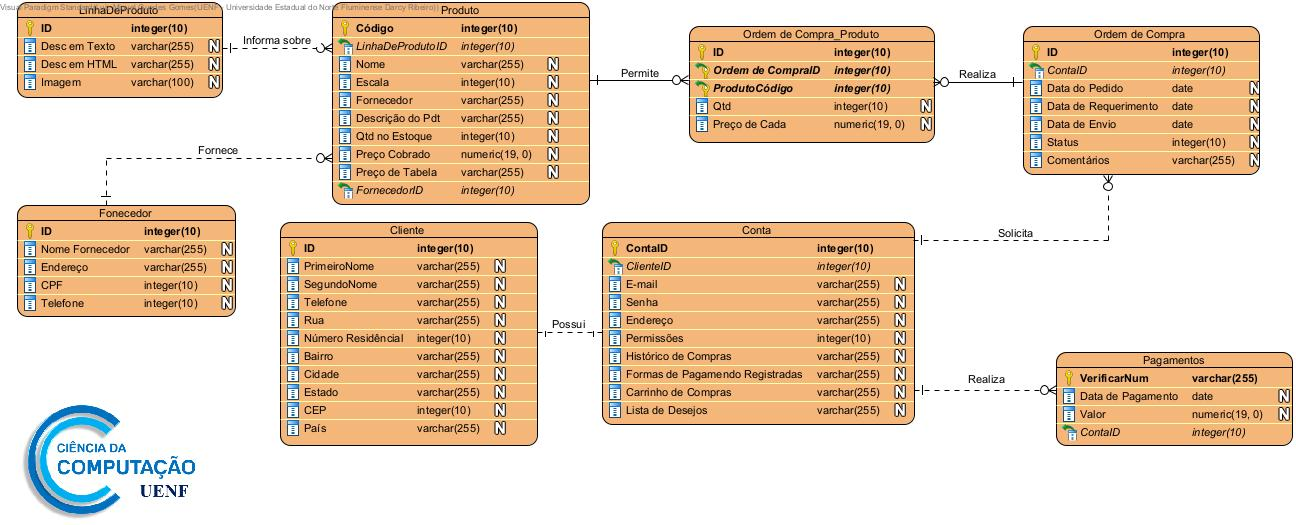
\includegraphics[width=14cm]{DFD7.jpg}
	    \caption{Diagrama de relacionamento: Cliente-Sistema: Ordem de Produto Online} 		
	    \label{tab:DFD7}
	 \end{center}
	 \end{table} 
	 
	 \begin{table}[H]
	 \begin{center}
	    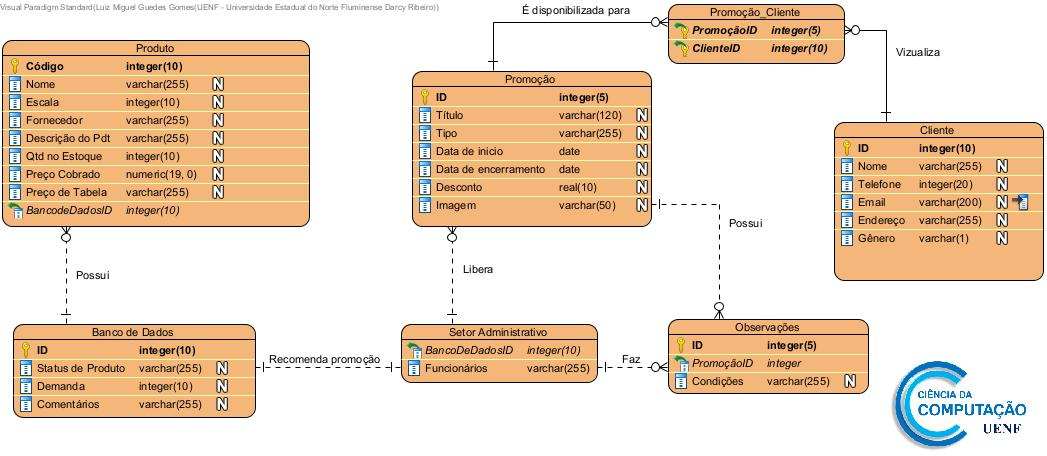
\includegraphics[width=14cm]{DFD8.jpg}
	    \caption{Diagrama de relacionamento: Promoções-Administração-Cliente} 		
	    \label{tab:DFD8}
	 \end{center}
	 \end{table} 
		
